\documentclass[11pt,a4paper]{article}

\usepackage[margin=2.2cm]{geometry}
\usepackage{amsmath}
\usepackage{booktabs}
\usepackage{graphicx}
\usepackage{xcolor}
\usepackage{array}
\usepackage{titlesec}
\usepackage[hidelinks]{hyperref}

\definecolor{spotter}{HTML}{064A56}
\definecolor{rule}{HTML}{9DAFB3}

\titleformat{\section}{\large\bfseries\color{spotter}}{\thesection.}{0.6em}{}
\titleformat{\subsection}{\normalsize\bfseries}{\thesubsection}{0.6em}{}
\titlespacing{\section}{0pt}{14pt}{6pt}
\titlespacing{\subsection}{0pt}{10pt}{4pt}

\setlength{\parskip}{5pt}
\setlength{\parindent}{0pt}
\renewcommand{\arraystretch}{1.15}

\graphicspath{{../scorer_results/}}

\newcommand{\key}[1]{\textbf{\color{spotter}#1}}

\begin{document}

\begin{center}
{\LARGE\bfseries\color{spotter} Freight Rate Prediction}\\[4pt]
{\large Machine Learning Engineer Assessment}\\[8pt]
{\small Talha Rashid \quad$\cdot$\quad
\href{https://github.com/rTalhaa/freight-rate-prediction}{github.com/rTalhaa/freight-rate-prediction}}
\end{center}

\vspace{2pt}
\hrule height 1.2pt
\vspace{10pt}

\section{Summary}

The task is a forward prediction: training covers 2025-01-01 to 2025-10-31, and
prediction covers 2025-11-01 to 2025-12-31. Every decision below follows from
that single fact.

Final model is a hybrid --- ridge on log-rate for global structure, LightGBM on
the residual. On the Sep--Oct holdout it scores \key{MAE \$49.84}, \key{MAPE
2.05\%}, \key{MedAPE 1.79\%} on clean rows.

Three results are worth more than the headline number:

\begin{itemize}\itemsep2pt
\item \key{About 1.39\% of training labels are corrupt.} Removing them is worth
\$38.40 of MAE --- the single largest intervention in the project.
\item \key{The time trend must not be extrapolated.} Three separate attempts to
project structure forward (Fourier terms, recency weighting, undamped trend) each
made results measurably worse and were removed.
\item \key{The December market forecast was audited, not assumed.} It was built
without touching the values \texttt{validation.csv} supplies for those dates, then
scored against them: accurate to 0.35\%.
\end{itemize}

\section{Data and Defects}

Seven defects, six of which appear in validation at the same rate --- so cleaning
lives in the prediction path, not just in training.

\begin{center}
\small
\begin{tabular}{@{}p{6.6cm}rrp{4.4cm}@{}}
\toprule
\textbf{Defect} & \textbf{Train} & \textbf{Valid.} & \textbf{Treatment}\\
\midrule
Corrupt labels (rpm $<1$ or $>4$) & 669 & --- & Drop, training folds only\\
Negative \texttt{weight} (sign flip) & 292 & 145 & \texttt{abs()}, not dropped\\
Missing \texttt{weight} & 300 & 165 & Median by equipment + flag\\
Missing \texttt{market\_index} & 374 & 249 & Same-day median + flag\\
\texttt{weight} censored at 47{,}500 & 1{,}191 & 297 & Keep value, flag\\
\texttt{distance} floored at 70 mi & 48 & 21 & Keep value, flag\\
Distorted city coordinates & 22 & 16 & Cap circuity at p99.9\\
\bottomrule
\end{tabular}
\end{center}

\subsection{The corrupt labels}

Rate-per-mile does not decay like a real tail --- it plateaus. There are 340 rows
above rpm 4, and still 145 above rpm 8, with only 23 rows in between. A genuine
heavy tail thins out; this does not. It is mirrored at the bottom by 329 rows
below rpm 1, roughly 0.7\% on each side, spread evenly across all ten months.
That is injected noise, not a market event. Example: Chattanooga to Atlanta, 98
miles, \$1{,}386.

These are dropped rather than winsorised, because they are corrupt rather than
extreme-but-real. Cross-validating the thresholds confirms the choice: MAE is
flat between bounds of 3.0 and 4.5, and no cleaning at all costs \$38.40.

\subsection{Sign flips are repaired, not discarded}

The absolute values of the 292 negative weights match the healthy distribution
almost exactly (median 31{,}822 against 31{,}494, both bounded 5{,}000--47{,}500).
They are recoverable, so dropping them would throw away 292 valid rows.

\subsection{One finding that changed the feature set}

\texttt{market\_index} correlates with rate at just 0.034 and looks like a decoy.
It is not --- distance was confounding it. Within every distance band, rate-per-mile
rises monotonically across market\_index quintiles with a consistent spread of
about 0.14. A raw correlation would have discarded a genuinely useful feature.

\section{Validation and Split Approach}

\subsection{The split is temporal, never random}

A random split lets September rates inform January predictions and posts a
flattering, meaningless score. The split is at 2025-08-31: fit on Jan--Aug
(37{,}951 rows), hold out Sep--Oct (9{,}523 rows).

The holdout is not merely later --- it reproduces the regime:

\begin{center}
\small
\begin{tabular}{@{}lr@{}}
\toprule
\textbf{Window} & \textbf{Mean \texttt{market\_index}}\\
\midrule
Fit (Jan--Aug) & 1.122\\
Holdout (Sep--Oct) & \key{0.926}\\
Real validation (Nov--Dec) & \key{0.927}\\
\bottomrule
\end{tabular}
\end{center}

The holdout lands within 0.001 of the real task while the fit window sits 21\%
above both. Validation is in a softer market than training, and a random split
would have averaged that away.

\subsection{Model selection uses rolling-origin folds}

One split is one draw. Selection runs on expanding-window folds with a
\key{61-day forward horizon} --- the same length as the real task, since the final
model trains through 31 October and predicts from 1 November. Training folds have
corrupt labels removed; \key{test folds keep theirs}, because the real scoring
will not be cleaned. Feature statistics are refitted per fold.

\subsection{Three guards against leakage}

\begin{enumerate}\itemsep2pt
\item \textbf{Cleaning parameters are fitted, then applied.} Imputation medians
come from the training window; they are never recomputed on validation.
\item \textbf{Lane statistics use strictly earlier dates.} An expanding mean that
merely excludes the row itself still lets same-day loads inform its feature ---
the same leak at one-day resolution. This was found and fixed late.
\item \textbf{The holdout is left contaminated.} Cleaning it would flatter the
reported metrics in exactly the way the real scoring will not.
\end{enumerate}

\subsection{A limitation of this design}

The temporal split reproduces the market regime faithfully, but \key{not the
unseen geography}. Validation contains 8 cities and 17.5\% of lanes never seen in
training; the Sep--Oct holdout contains 22 such rows, 0.2\%, because both windows
cover the same 64 cities.

This was measured separately by holding 8 random cities out of training across
three trials: unseen geography costs \key{+18.6\% MAPE} (2.45\% against 2.06\%).
Degradation rather than failure, because an unseen city still has coordinates, a
distance and an equipment type --- which is why coordinates, not lane statistics,
carry the fallback.

\section{Features: What Worked and What Failed}

\begin{center}
\small
\begin{tabular}{@{}lrrrr@{}}
\toprule
\textbf{Features} & \textbf{n} & \textbf{MAE} & \textbf{MAPE} & \textbf{Bias}\\
\midrule
Base & 13 & 161.43 & 7.00 & $-100.38$\\
+ time & 14 & 118.31 & 5.37 & $-26.64$\\
+ geography & 25 & 108.76 & 4.82 & $-26.88$\\
+ lane history & 31 & \key{106.99} & \key{4.67} & $-31.63$\\
+ interactions & 36 & 108.63 & 4.71 & $-34.43$\\
\bottomrule
\end{tabular}
\end{center}

Interactions were dropped despite the market\,$\times$\,distance effect being real:
ridge already captures it through log-distance, so the explicit terms only added
variance. A real effect is not automatically a useful feature.

\subsection{Annual Fourier terms made things worse}

Seasonality is normally modelled with Fourier terms. Here they were actively
harmful --- MAE \$118 to \$175, holdout bias $-$\$27 to $-$\$115.

The cause is measurable: over an eight-month window,
$\mathrm{corr}(\texttt{trend\_days}, \texttt{annual\_cos}) = -0.92$. The harmonics
are nearly collinear with the trend, so ridge splits the coefficient between them.
That is harmless in-sample and diverges the moment prediction moves past the edge
of the window. Month dummies were never an option: November and December do not
appear in training at all.

\subsection{Recency weighting made things worse}

Exponentially decayed sample weights were the intuitive fix for the drift. Tested
across nine half-lives from 21 to 365 days, every one was worse on both MAE and
bias. Once the trend is an explicit feature, down-weighting old rows removes
information without adding any.

\section{Model}

\begin{center}
\small
\begin{tabular}{@{}lrrrr@{}}
\toprule
\textbf{Model} & \textbf{MAE} & \textbf{MAPE} & \textbf{MedAPE} & \textbf{Bias}\\
\midrule
\key{Hybrid} & \key{110.45} & \key{4.67} & 2.02 & $+20.95$\\
LightGBM & 114.65 & 4.79 & 1.94 & $-19.54$\\
Ridge & 115.66 & 4.95 & 2.32 & $+18.38$\\
\bottomrule
\end{tabular}
\end{center}

Neither model alone wins, and the reason is structural. \key{Tree splits cannot
emit a value outside their training range}, so no tree can follow the time trend
past the end of training. A task defined by forward extrapolation gives the linear
model an advantage that tuning cannot close.

So the job is split. \textbf{Stage one:} ridge on log-rate over the full feature
set, carrying the trend --- the only component that must extrapolate --- linearly.
\textbf{Stage two:} LightGBM fits the stage-one residual using features with
\key{no time component at all}, capturing non-linear structure without ever being
asked for a value outside its range.

Confirmed on six folds at a 30-day horizon: hybrid 98.59 against ridge 105.82.
Metrics are reported as a family throughout because the scoring metric is not
published --- RMSE is driven by long expensive loads, MAPE by short cheap ones,
and they rank models differently.

\subsection{The trend is deliberately not extrapolated}

Past the last training date the trend input is damped:
$t_{\text{eff}} = t_{\max} + \varphi\,(t - t_{\max})$. Sweeping $\varphi$ gave a
monotonic result, with $\varphi = 0$ --- freezing the level --- winning every
criterion:

\begin{center}
\small
\begin{tabular}{@{}lrrrr@{}}
\toprule
$\varphi$ & \textbf{Mean MAE} & \textbf{Worst fold} & \textbf{Max $|$bias$|$} & \textbf{Spread}\\
\midrule
1.0 & 110.74 & 138.31 & 84.21 & 42.82\\
0.5 & 106.87 & 126.44 & 69.99 & 34.10\\
\key{0.0} & \key{104.80} & \key{116.01} & \key{55.88} & \key{23.32}\\
\bottomrule
\end{tabular}
\end{center}

Selection criteria were set to prefer worst-fold MAE and maximum bias over the
average, on the grounds that the failure mode is variance across regimes. The
criteria did not disagree.

The interpretation matters more than the number. Dropping time features entirely
scores 134.34; keeping the trend but refusing to project it scores 104.80.
\key{The trend earns its place by de-confounding historical rates, not by
predicting future ones.} Rate-per-mile rose through June and then fell --- a slope
fitted across that turn adds variance and no information.

\section{December Chart}

\begin{center}
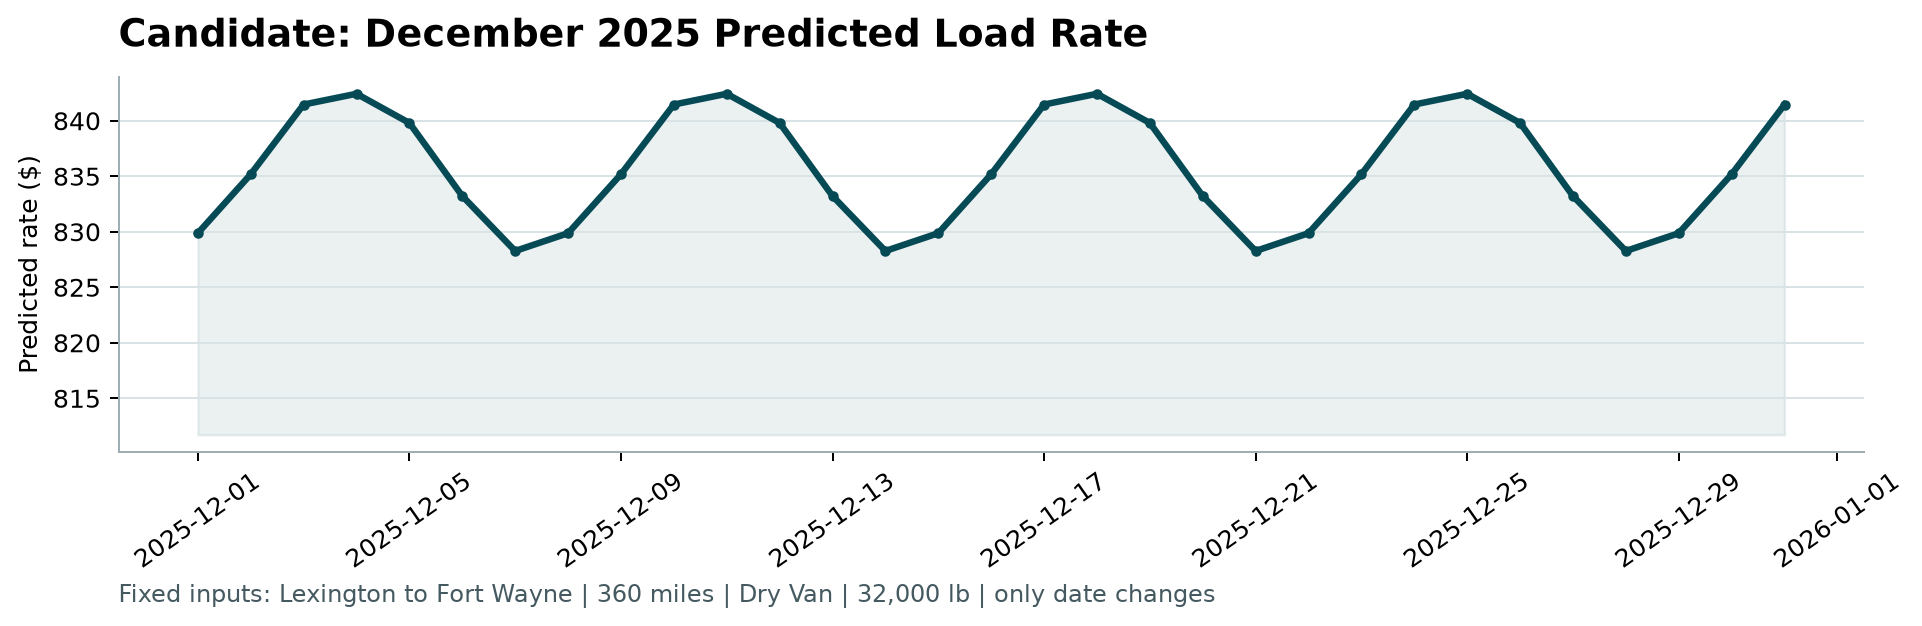
\includegraphics[width=\textwidth]{candidate_december.png}
\end{center}

The chart file supplies only seven columns: no coordinates, no
\texttt{market\_index}, no \texttt{quote\_signal}. Two different gaps, handled
differently.

\textbf{Coordinates are a fact.} Every city maps to exactly one lat/lon,
identically in train and validation, so looking up Lexington and Fort Wayne
recovers a static property.

\textbf{Market features are a forecast.} \texttt{validation.csv} does contain them
for December dates, and joining them would have been simple. It was not done:
\key{a deployed quoting model pricing a future load would not know that date's
market index}. They are forecast from training data alone, and the withheld values
are used afterwards to score the forecast instead.

\begin{center}
\small
\begin{tabular}{@{}lrrrr@{}}
\toprule
\textbf{Series} & \textbf{Forecast} & \textbf{Actual} & \textbf{Error} & \textbf{vs naive}\\
\midrule
\texttt{market\_index} & 0.9376 & 0.9344 & \key{$+0.35\%$} & 93.5\% better\\
\texttt{quote\_signal} & 2.0587 & 2.0475 & $+0.54\%$ & 14.6\% better\\
\bottomrule
\end{tabular}
\end{center}

Ranges match too --- actual \texttt{market\_index} spans [0.8306, 1.0445] against a
forecast [0.8426, 1.0387] --- so the weekly amplitude is right, not just the level.

The forecaster is a trailing level plus a weekly profile, with window length
chosen by backtesting the last 61 days of training, never against December. The
two series needed opposite treatment: \texttt{market\_index} has a dominant weekly
cycle (lag-7 autocorrelation 0.97) and takes a 7-day window with a weekday profile;
\texttt{quote\_signal} has none and takes a 56-day window, flat.

\subsection{Reading the chart}

Predictions run \$828.27 to \$842.43, mean \$835.72. The historical anchor --- 32
training loads on this exact lane --- averages \$856.59, so predictions sit 2.4\%
below history, consistent with December's softer market.

The line repeats every seven days because the level is flat by design and the
weekly cycle is the only varying input. That repetition is a consequence of not
extrapolating the trend, not an artefact. Given the audit above, the flat level
was the correct call: inventing December drift the data cannot support is the
mistake this project measured three separate times.

\section{Results and Limitations}

\begin{center}
\small
\begin{tabular}{@{}lr@{}}
\toprule
\textbf{Stage} & \textbf{MAE (61-day CV)}\\
\midrule
No cleaning & 143.20\\
Flat \$/mile baseline & 274.96\\
Ridge, base features & 118.34\\
+ time, geography, lane & 106.99\\
Hybrid + damped trend & \key{104.80}\\
\bottomrule
\end{tabular}
\end{center}

On the Sep--Oct holdout, clean rows: \key{MAE \$49.84, MAPE 2.05\%, MedAPE 1.79\%}.
MAPE is flat across distance bands (1.83--2.31\%), so there is no short-haul
weakness. Flatbed is the weakest class at 2.56\% against Dry Van's 1.88\%.

\subsection{Known limitations}

\begin{itemize}\itemsep3pt
\item \textbf{No holiday effects.} Training ends in October, so 25 December prices
as an ordinary Thursday. A hand-specified holiday bump was rejected: there is no
in-sample evidence for its size, and every imposed structure this data could not
support has made results worse.
\item \textbf{Bias is roughly $-1.8\%$ of rate}, uniform across every segment.
A level effect rather than a structural one, but not eliminated.
\item \textbf{$\varphi = 0$ sits at the edge of its grid}, so the data prefers the
most conservative option tested rather than an interior optimum, on three folds.
\item \textbf{Error nearly doubles across the horizon} --- MAE \$33 in the first
fortnight against \$64 in the last. Late-December predictions are inherently
weaker. That is a property of the task, not something the model removes.
\item \textbf{Unseen geography costs $+18.6\%$ MAPE}, measured by simulation
because the temporal holdout cannot test it.
\end{itemize}

\vspace{6pt}
\hrule height 0.6pt
\vspace{6pt}

{\small Full evidence in the repository: seven documents under \texttt{docs/},
each backed by a runnable script under \texttt{notebooks/}. Reproduce with
\texttt{python -m src.predict}.}

\end{document}
